\subsection{Fit dos tempos entre chegadas para cada mês} 
\label{section: fit-arrivals}
Conforme atestado no teste de hipóteses apresentado na Figura \ref*{fig: ks-arrivals}, o tempo entre as chegadas das ligações muda mês a mês, sendo necessário representar o intervalo entre as chegadas com diferentes distribuições de probabilidade ao longo do tempo em nosso modelo de simulação. A distribuição exponencial é a mais adequada para modelar os dados em todos os meses, visto que apresenta pequenos erros e maiores valores $p$ em relação às demais distribuições.

\subsubsection*{Janeiro}
No primeiro mês do ano, o teste de aderência de Kolgomogorov-Smirnov indica que a distribuição que melhor representa os valores dos tempos entre chegadas é a exponencial com média 248,6240 segundos. A Figura \ref*{fig: fit-janeiro} apresenta o resumo dos testes realizados.

\begin{figure}[H]
    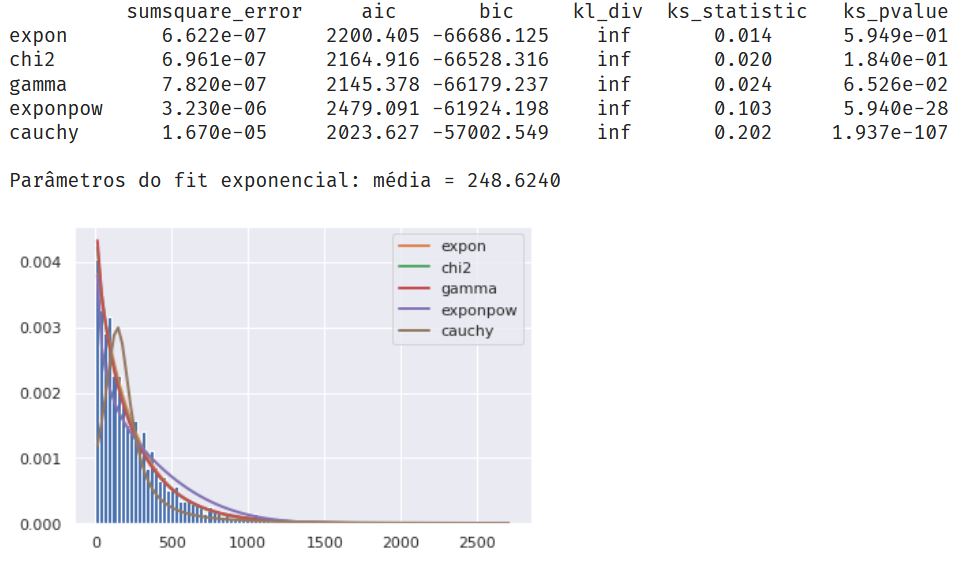
\includegraphics[scale=0.8]{analise-de-dados/fit/fit-janeiro.png}
    \caption{Teste de aderência dos tempos entre chegadas para o mês de janeiro}
    \label{fig: fit-janeiro}
\end{figure}

\subsubsection*{Fevereiro}
No mês de fevereiro, o teste de aderência indica que a distribuição que melhor representa os valores dos tempos entre chegadas é a exponencial com média 231,8853 segundos. A Figura \ref*{fig: fit-fevereiro} apresenta o resumo dos testes realizados.

\begin{figure}[H]
    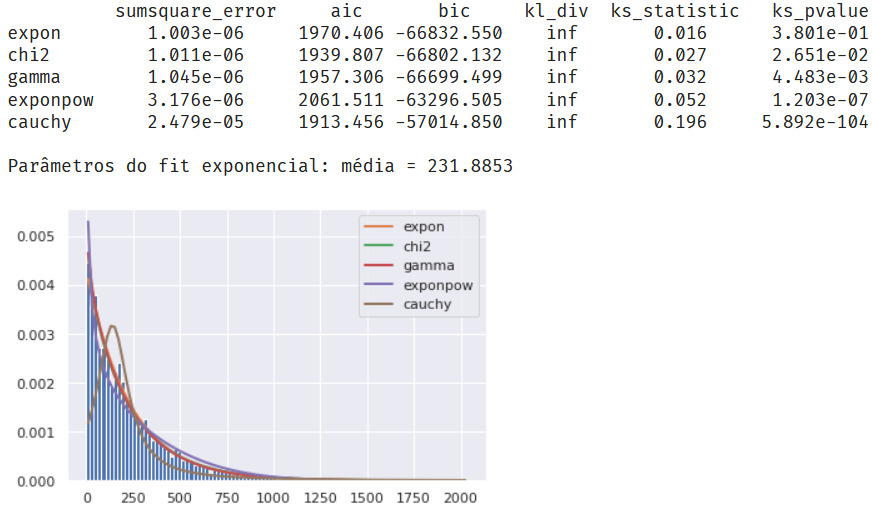
\includegraphics[scale=0.8]{analise-de-dados/fit/fit-fevereiro.png}
    \caption{Teste de aderência dos tempos entre chegadas para o mês de fevereiro}
    \label{fig: fit-fevereiro}
\end{figure}

\subsubsection*{Março}
No mês de março, o teste de aderência indica que a distribuição que melhor representa os valores dos tempos entre chegadas é a exponencial com média 226,2098 segundos. A Figura \ref*{fig: fit-marco} apresenta o resumo dos testes realizados.

\begin{figure}[H]
    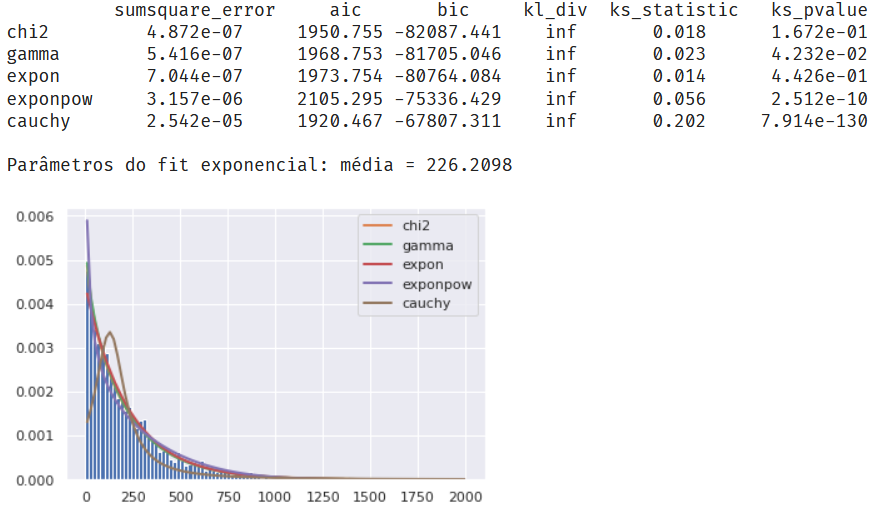
\includegraphics[scale=0.8]{analise-de-dados/fit/fit-marco.png}
    \caption{Teste de aderência dos tempos entre chegadas para o mês de março}
    \label{fig: fit-marco}
\end{figure}

\subsubsection*{Abril}
No mês de abril, o teste de aderência indica que a distribuição que melhor representa os valores dos tempos entre chegadas é a exponencial com média 214,1724 segundos. A Figura \ref*{fig: fit-abril} apresenta o resumo dos testes realizados.

\begin{figure}[H]
    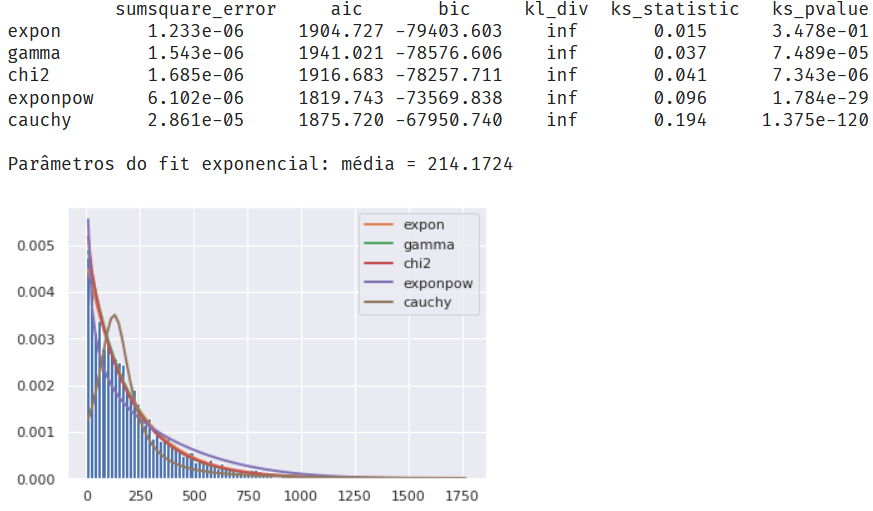
\includegraphics[scale=0.8]{analise-de-dados/fit/fit-abril.png}
    \caption{Teste de aderência dos tempos entre chegadas para o mês de abril}
    \label{fig: fit-abril}
\end{figure}

\subsubsection*{Maio}
No mês de maio, o teste de aderência indica que a distribuição que melhor representa os valores dos tempos entre chegadas é a exponencial com média 206,9737 segundos. A Figura \ref*{fig: fit-maio} apresenta o resumo dos testes realizados.

\begin{figure}[H]
    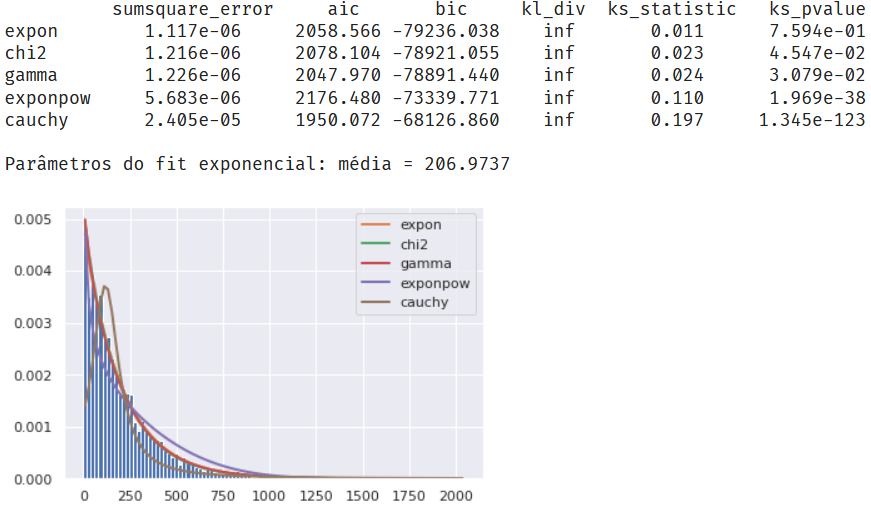
\includegraphics[scale=0.8]{analise-de-dados/fit/fit-maio.png}
    \caption{Teste de aderência dos tempos entre chegadas para o mês de maio}
    \label{fig: fit-maio}
\end{figure}

\subsubsection*{Junho}
No mês de junho, o teste de aderência indica que a distribuição que melhor representa os valores dos tempos entre chegadas é a exponencial com média 195,4312 segundos. A Figura \ref*{fig: fit-junho} apresenta o resumo dos testes realizados.

\begin{figure}[H]
    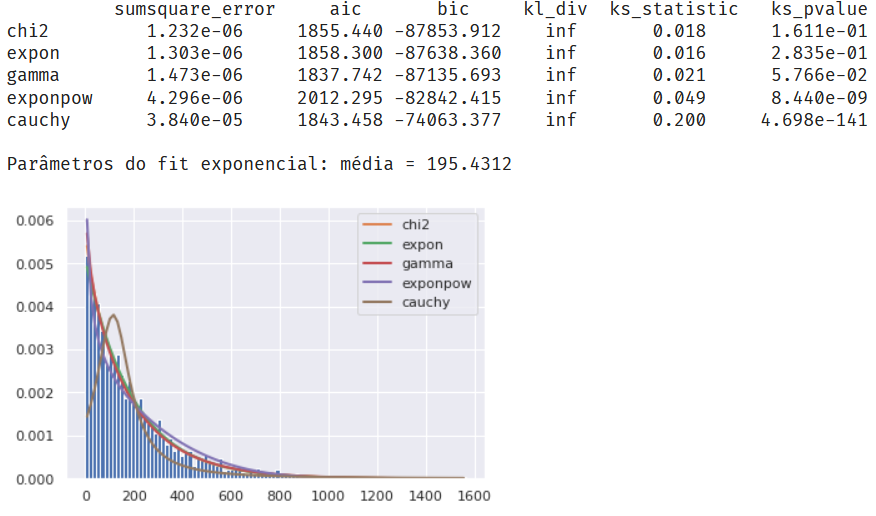
\includegraphics[scale=0.8]{analise-de-dados/fit/fit-junho.png}
    \caption{Teste de aderência dos tempos entre chegadas para o mês de junho}
    \label{fig: fit-junho}
\end{figure}

\subsubsection*{Julho}
No mês de julho, o teste de aderência indica que a distribuição que melhor representa os valores dos tempos entre chegadas é a exponencial com média 180,2765 segundos. A Figura \ref*{fig: fit-julho} apresenta o resumo dos testes realizados.

\begin{figure}[H]
    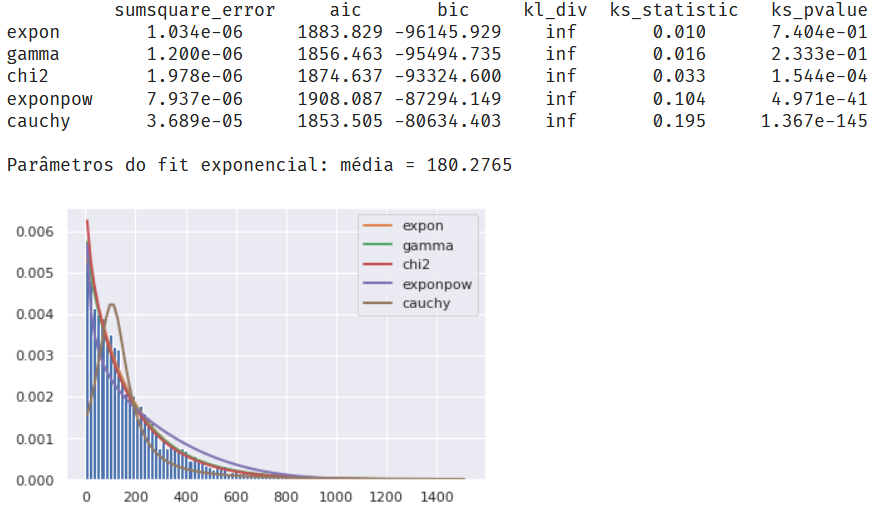
\includegraphics[scale=0.8]{analise-de-dados/fit/fit-julho.png}
    \caption{Teste de aderência dos tempos entre chegadas para o mês de julho}
    \label{fig: fit-julho}
\end{figure}

\subsubsection*{Agosto}
No mês de agosto, o teste de aderência indica que a distribuição que melhor representa os valores dos tempos entre chegadas é a exponencial com média 171,8725 segundos. A Figura \ref*{fig: fit-agosto} apresenta o resumo dos testes realizados.

\begin{figure}[H]
    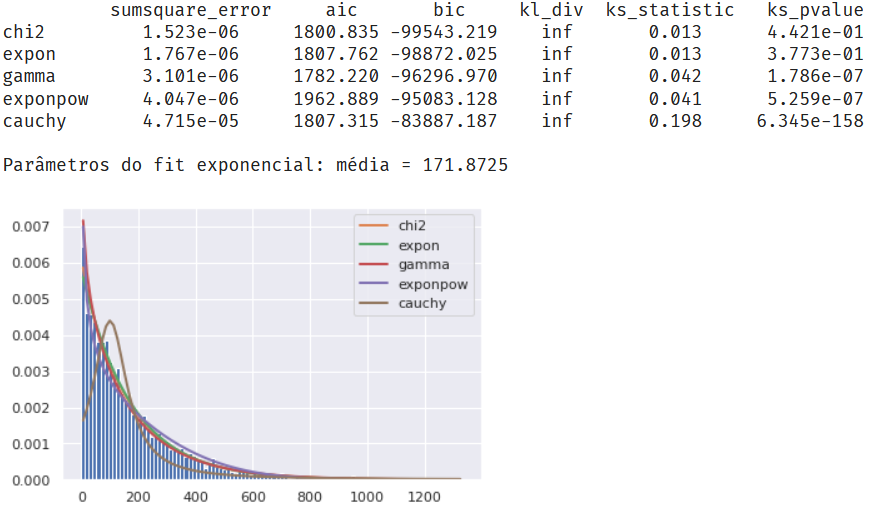
\includegraphics[scale=0.8]{analise-de-dados/fit/fit-agosto.png}
    \caption{Teste de aderência dos tempos entre chegadas para o mês de agosto}
    \label{fig: fit-agosto}
\end{figure}

\subsubsection*{Setembro}
No mês de setembro, o teste de aderência indica que a distribuição que melhor representa os valores dos tempos entre chegadas é a exponencial com média 156,4994 segundos. A Figura \ref*{fig: fit-setembro} apresenta o resumo dos testes realizados.

\begin{figure}[H]
    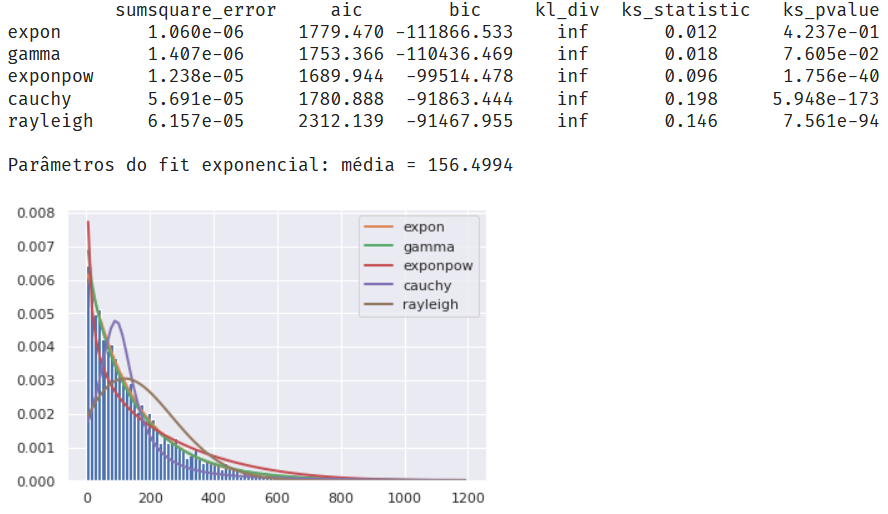
\includegraphics[scale=0.8]{analise-de-dados/fit/fit-setembro.png}
    \caption{Teste de aderência dos tempos entre chegadas para o mês de setembro}
    \label{fig: fit-setembro}
\end{figure}

\subsubsection*{Outubro}
No mês de outubro, o teste de aderência indica que a distribuição que melhor representa os valores dos tempos entre chegadas é a exponencial com média 149,7512 segundos. A Figura \ref*{fig: fit-outubro} apresenta o resumo dos testes realizados.

\begin{figure}[H]
    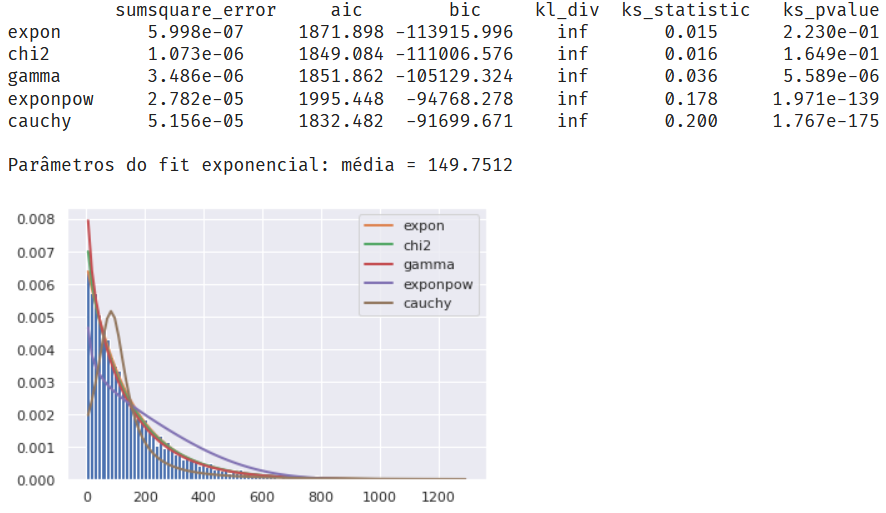
\includegraphics[scale=0.8]{analise-de-dados/fit/fit-outubro.png}
    \caption{Teste de aderência dos tempos entre chegadas para o mês de outubro}
    \label{fig: fit-outubro}
\end{figure}

\subsubsection*{Novembro}
No mês de novembro, o teste de aderência indica que a distribuição que melhor representa os valores dos tempos entre chegadas é a exponencial com média 139,9637 segundos. A Figura \ref*{fig: fit-novembro} apresenta o resumo dos testes realizados.

\begin{figure}[H]
    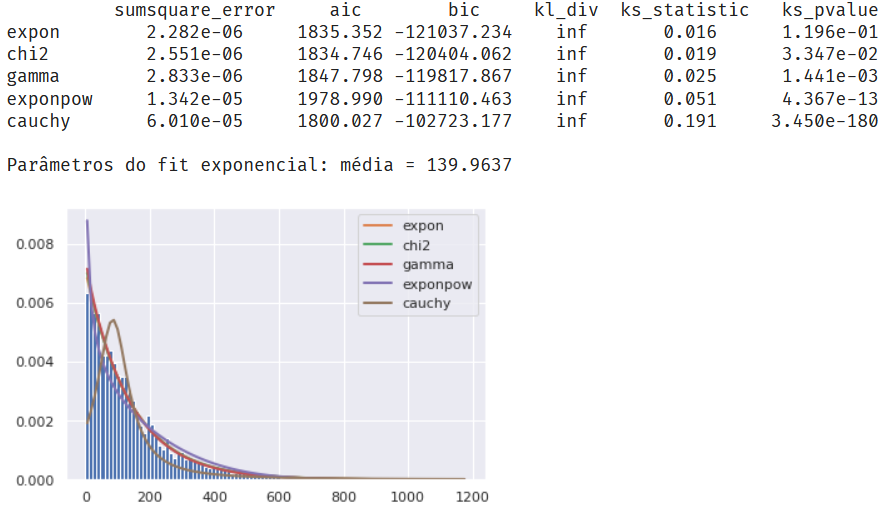
\includegraphics[scale=0.8]{analise-de-dados/fit/fit-novembro.png}
    \caption{Teste de aderência dos tempos entre chegadas para o mês de novembro}
    \label{fig: fit-novembro}
\end{figure}

\subsubsection*{Dezembro}
No mês de dezembro, o teste de aderência indica que a distribuição que melhor representa os valores dos tempos entre chegadas é a exponencial com média 131,3733 segundos. A Figura \ref*{fig: fit-dezembro} apresenta o resumo dos testes realizados.

\begin{figure}[H]
    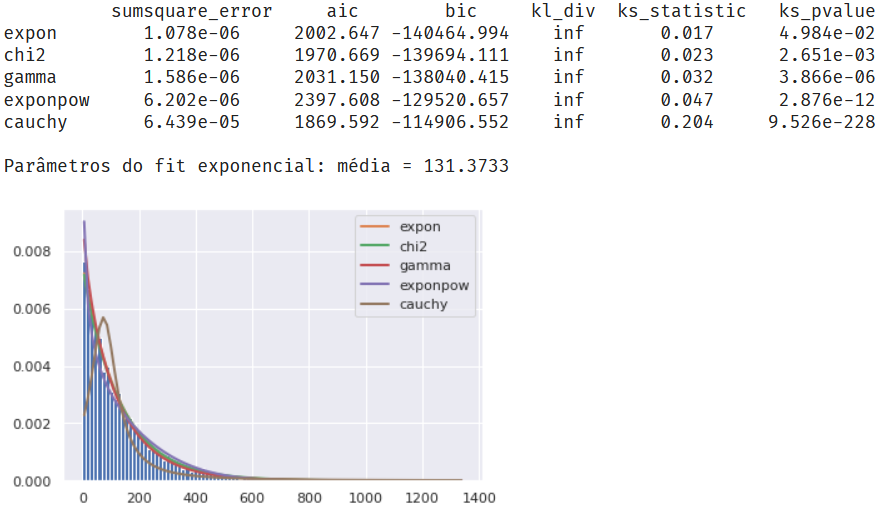
\includegraphics[scale=0.8]{analise-de-dados/fit/fit-dezembro.png}

    \caption{Teste de aderência dos tempos entre chegadas para o mês de dezembro}
    \label{fig: fit-dezembro}
\end{figure}